\section{Global structure}
The figure \ref{fig: Tree view of the Numerics directories} represents the architecture of \ac{numerics}'s directories.
	\begin{figure}
	\begin{center}
	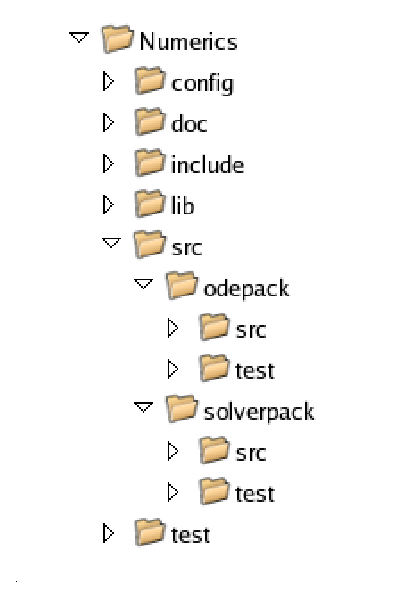
\includegraphics[scale=1.2, clip]{figure/NumericsDesign.eps}
	\caption{Tree view of the Numerics directories}
	\label{fig: Tree view of the Numerics directories}
	\end{center}
	\end{figure}




\begin{ndr}
put everywhere the main methods of the different modules\\
=> listing of the methods\\
\\
even if it's not very nice, it's a way to show the main methods that we can use
\end{ndr}


\section{Detailed design}
\subsection{\acs{lapack}}
%\begin{ndr}
%put here the funcitons used from LAPACK
%\end{ndr}
See the website dedicated to \ac{lapack} 
\begin{verbatim}( http://www.netlib.org/lapack/ ).\end{verbatim}
More details on the content of \ac{lapack} are available in this page 
\begin{verbatim}( http://www.netlib.org/lapack/lug/node19.html ).\end{verbatim}


\subsection{MP solverpack}
c.f. \ac{numerics} source code documentation generated by DOxygen.
\begin{ndr}
put here the information of the "poster" of solverpack
\end{ndr}


\subsection{\ac{ode} pack}
The functionalities given by \ac{ode} pack with \ac{numerics} are described in the documentation generated by DOxygen.
It correspond to the section called ...
\begin{ndr}
put the name of the .h of the C interface for ODE pack
\end{ndr}
